\documentclass[titlepage]{report}
\usepackage[italian]{babel}
\usepackage[babel]{csquotes}
\usepackage[a4paper,left=2cm,bottom=2cm,right=2cm,top=2.5cm]{geometry}
\usepackage[style=numeric-comp,useprefix,hyperref,backend=bibtex,natbib,sorting=none]{biblatex}
\usepackage{subcaption}
\usepackage{url}
\usepackage{graphicx} 			% pacchetto per inserire immagini
\usepackage{sidecap}			% pacchetto delle didascalie laterali
\usepackage{setspace}			% pacchetto per modificare interlinea
\usepackage{textcomp} 			% pacchetto per simboli unicode
\usepackage{float}
\usepackage{hyperref}
\usepackage{fancyhdr}
\usepackage[nowrite,infront,standard,swapnames]{frontespizio}

\begin{document}
	
\hypersetup{
	linkbordercolor={1 1 1},
}

\begin{frontespizio}
	\Universita {Brescia}
	\Logo [3cm]{Logo_unibs.pdf}
	\Dipartimento {Ingengeria dell'Informazione}
	\Corso [Laurea magistrale]{Ingegneria Elettronica}
	\Annoaccademico {2020--2021}
	\Titoletto{Progetto di Sistemi Elettronici Analogici}
	\Titolo {Circuito per la generazione del tono \\ (sinusoidale a frequenza variabile) per Theremin}
	\Sottotitolo{Progetto n°17}
	\NCandidati{Autori}
	\Candidato [706005]{Luca Brescia}
	\Candidato [89521]{Simone Pezzottini}
\end{frontespizio}
	
\tableofcontents

\chapter*{Obiettivo}
	\label{ch:Scope}
	\addcontentsline{toc}{chapter}{Obiettivo}
	\large Realizzazione di un tono a frequenza variabile nello spettro delle frequenze udibili [$20Hz - 20kHz$] utilizzando un VCO e una capacità variabile con il movimento di una mano seguendo lo schema a blocchi mostrato in \textit{Figura \ref{fig:Schema_Assegnazione}}. Il segnale modulato avrà un range di frequenze elevato, di conseguenza andrà mixato ad una sinusoide a frequenza determinata, per riportare lo spettro del segnale nel range delle frequenze udibili, e opportunamente filtrato per eliminare le componenti indesiderate.
	\\
	\\
	\begin{figure}[h]
		\centering
		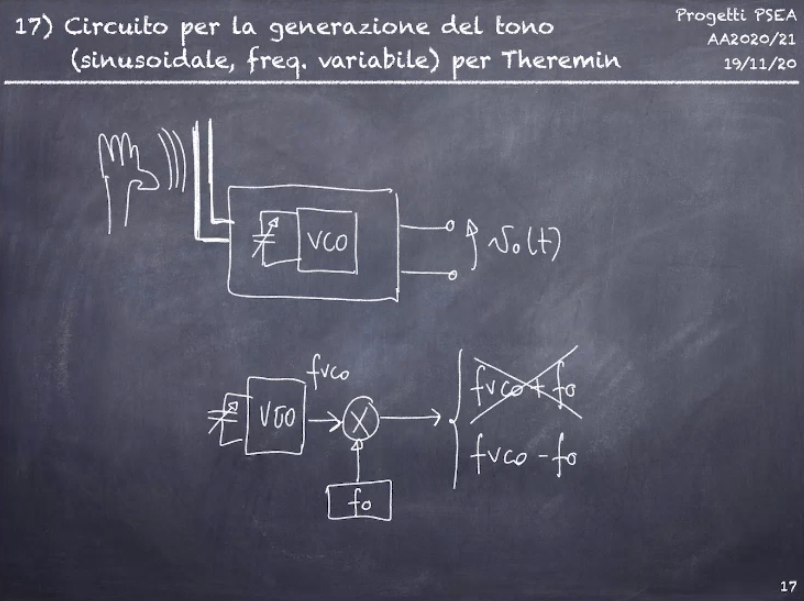
\includegraphics[scale=0.5]{Immagini/Schema_progetto_17.png}
		\caption{Schema generale di funzionamento di un circuito per la realizzazione di un tono.}
		\label{fig:Schema_Assegnazione}
	\end{figure}

	 In generale lo schema richiesto per la realizzazione del progetto potrebbe essere il seguente:
	 
	\begin{figure}[htbp]
		\centering
		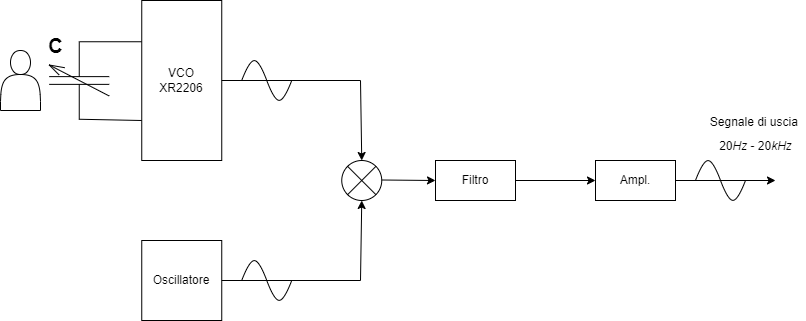
\includegraphics[scale=0.5]{Immagini/Schema Generale PSEA.png}
		\caption{Shema a blocchi generale del progetto}
		\label{fig: schema a blocchi generico}
	\end{figure}	


\newpage

	
\chapter{Scelta dei componenti}
	\label{ch:Scelta_componenti}
	I blocchi minimi necessari alla realizzazione di questo progetto sono:
	
	\begin{enumerate}
		\item Oscillatore controllato in tensione $(VCO)$;
		\item Moltiplicatore analogico;
		\item Oscillatore a frequenza fissata;
		\item Filtro passa basso.
		\item Prova di una modifica.
	\end{enumerate}
	
	\noindent La scelta dei componenti è stata fatta considerando le caratteristiche del segnale da generare. In particolare, volendo realizzare uno shift in frequenza, vi è la necessità di lavorare con integrati con una banda passante adeguata.
	Avendo a disposizione una serie limitata di componenti si è deciso di utilizzare i seguenti:
	
	\begin{enumerate}
		\item l'oscillatore monolitico XR2206 come VCO;
		\item Il moltiplicatore analogico AD633 per lo shift frequenziale;
		\item L'amplificatore operazionale $LF356N$ per la realizzazione dell oscillatore a ponte di Wien per la generazione di una sinusoide di riferimento;
		\item L'amplificatore $LF356P$ per la realizzazione di filtro passa basso.
		\item L'amplificatore $UA741$ per la realizzazione dei filtri passa alto.
	\end{enumerate}
	
	
\section{Amplificatori operazionali LF353, LF356 e uA741}
\label{sec:OpAmp}
	La scelta di questi componenti tra quelli disponibili è stata fatta principalmente per le bande bassanti dei dispositivi.
	\\ Sono necessari componenti a banda elevata poiché, come risulta dal capitolo \ref{ch:Risultati}, si deve lavorare con frequenze dell'ordine delle centinaia di kHz.
	
	 \noindent Infatti le bande in gioco sono di circa 3MHz per LF353P mentre 5MHz per LF356N. Ad esempio, l'UA741 ha una GBP di 1 MHz tipico. I primi due operazionali sono stati scelti per:
	
	\begin{enumerate}
		\item LF356N per l'oscillatore armonica fondamentale 
		\item LF353P per il filtro passa basso del 4o ordine. 
	\end{enumerate}
	
	
	\noindent Importante osservare che l'LF353P ha al suo interno due amplificatori operazionali per cui è stato scelto per la realizzazione del filtro del 4o ordine in modo da ridurre il numero di integrati per la realizzazione del dispositivo. Inoltre, l'LF356N, avente una GBP maggiore (5MHz), permette di generare sinusoidi con un range di freuenze maggiore, altro motivo per cui si sono scelti i componenti come spiegato sopra.
	L'UA741 viene impiegato come filtro attivo passa alto del primo ordine $(e come amplificatore finale)$ per togliere le componenti inferiori a 10Hz come richiesto dal progetto e sfruttare contemporaneamente la banda passante ridotta del dispositvo al fine di attenuare le alte frequenze indesiderate.

	\noindent I motivi per cui le frequenze in gioco risultino essere elevate sono indicate nel capitolo \ref{ch:Risultati}.

	
\section{Oscillatore monolitico XR2206}
	\label{sec:XR2206}
	
	Si è scelto di utilizzare $XR2206$ perchè permette la generazione di diverse forme d'onda sinusoidali, onde quadre, rampe, onde triangolari ed impunsi garantendo un'alta precisione, stabilità e distorsione. L'ampiezza e la frequenza dei segnali in uscita è direttamente modulabile dall'integrato, gestendo opportunamente gli ingressi. La gamma di frequenze generabili va dai 0.01 $HZ$ a 1 $MHz$, quindi perfetto per le specifiche richieste dal progetto. 
	In \textit{Figura \ref{fig:sch_xr2206}} è mostrato lo schema a blocchi del componente.
	
	\begin{figure}[h]
		\centering
		\subfloat[][\emph{Schema dei collegamenti interni}]
		{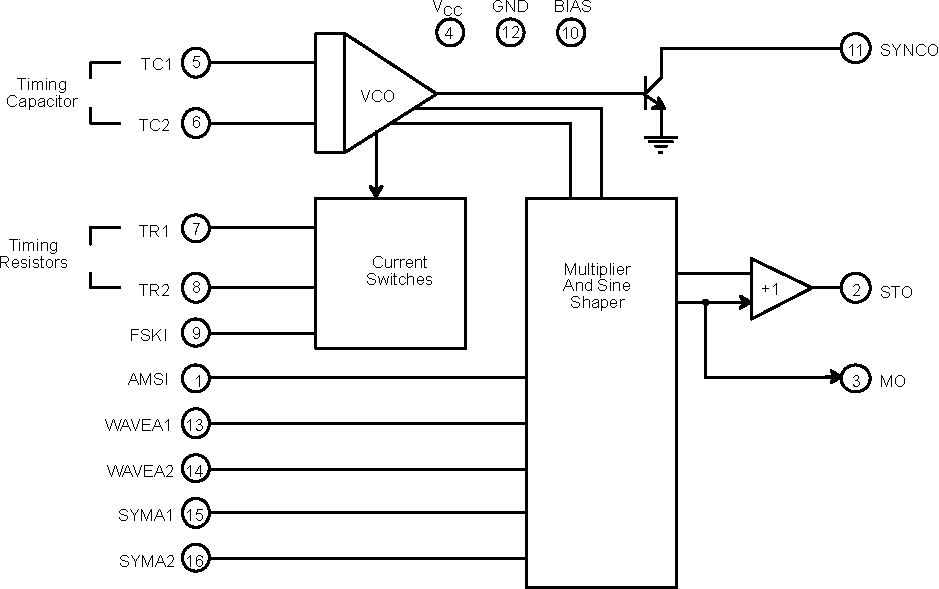
\includegraphics[width=.40\textwidth]{Immagini/schema_blocchi_xr2206.pdf}} \qquad
		\subfloat[][\emph{Descrizione in dettaglio dei pin}]
		{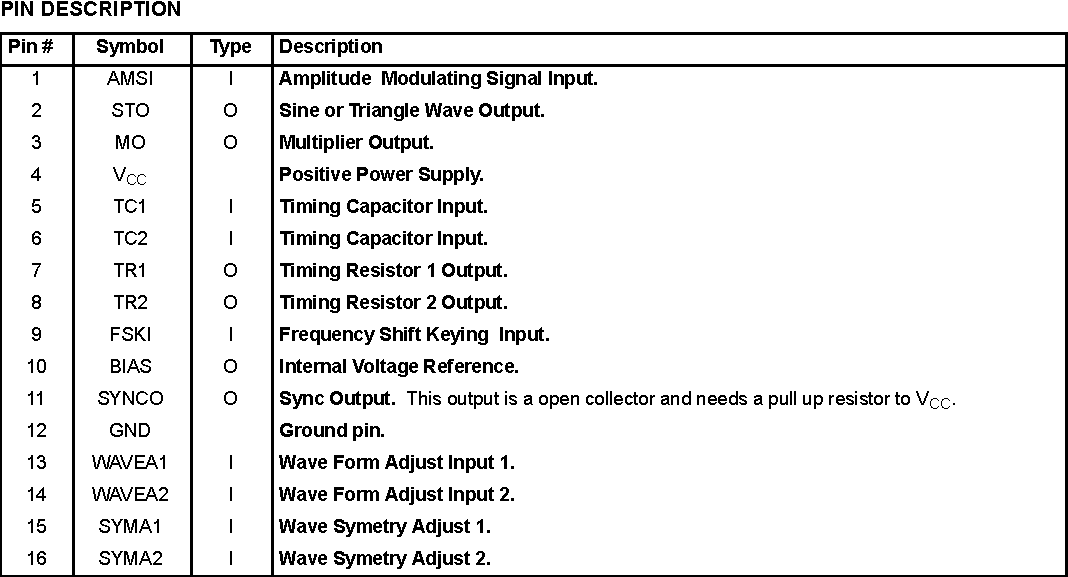
\includegraphics[width=.5\textwidth]{Immagini/schema_blocchi_pinout_xr2206.pdf}} \\
		\caption{Schema a blocchi dell'oscillatore monolitico XR2206}
		\label{fig:sch_xr2206}
	\end{figure}

	La frequenza di oscillazione può essere determinata agendo sulla capacità o sulla resistenza equivlente collegate ai pin opportuni del componente, come riportato nel capitolo \ref{ch:scelte}.
	
	
\section{Moltiplicatore analogico AD633}
	\label{sec:AD633}
	La scelta del moltiplicatore analogico o mixer è stata obbigata in quanto non erano presenti altri componenti del genere a disposizione.
	Tuttavia garantisce delle buone prestazioni permettendo di restare nelle specifiche di progetto.
	Infatti, possiede elevate impedenze d'ingresso sia sugli ingressi differenziali $X$ e $Y$, che sull'ingersso sommatore $Z$. Una bassa impedenza d'uscita che permette quindi di disaccoppiare la parte a monte del circuito con quella che si trova a valle. Lavora con una larghezza di banda pari ad 1 $MHz$ e uno slew rate pari a 20 $V/\mu S$. 
	Si può notare, come mostrano in figura \ref{fig:sch_ad633}, che il componete inizia a tagliare ad una frequenza inferiore ripetto alla banda passante teorica indicata, tagliando intorno ai 500 $kHz$.
	Tuttavia, dal punto di vista teorico, questo non impone una limitazione ai fini del progetto.

	\begin{figure}[H]
		\centering
		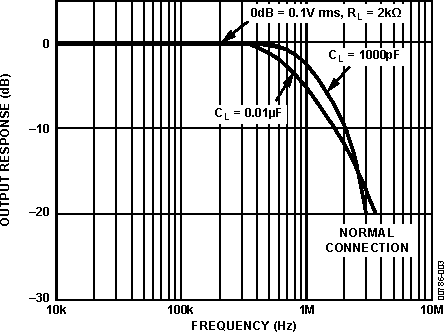
\includegraphics[scale=1]{Immagini/ad633_bp.pdf}
		\caption{Banda passante del moltiplicatore analogico AD633}
		\label{fig:sch_ad633}
	\end{figure}

	
	\noindent La figura \ref{fig: AD633 schema a blocchi} mostra sia il pinout che lo schema  blocchi interno dell'$AD6333$. Il segnale in uscita dal mixer si calcola con la seguente formula:

	\begin{equation}
		\label{eq: funzione trasferimeto AD633}
		W = \frac{(X1 - X2)(Y1 - Y2)}{10 [V]}  + Z 
	\end{equation}

	Come si può notare dalla formula in segnale viene attenuato di un fattore 10 $V$, quindi sarà necessaria una compensazione negli stadi successivi. 

	\noindent Analizzando il caso che gli ingressi X2, Y2 e Z collegti a massa, ovvero che diano contributo nullo. L'equazione \ref*{eq: funzione trasferimeto AD633} diventa:


	\begin{equation}
		\label{eq: prodotto sinusoidi AD633}
		W = \frac{X1 * Y1}{10 [V]}
	\end{equation}


	Ora si consideri che i due ingressi siano sinusoidali:


	\begin{equation}
		\label{eq: X1 sinusoidale}
		X1 = A\sin (\omega _1t + \varphi _1)
	\end{equation}
	\begin{equation}
		\label{eq: XY sinusoidale}
		Y1 = B\sin (\omega _2t + \varphi _2)
	\end{equation}
	\begin{equation}
		\label{eq:prodotto sinusoidi con fase}
		W = \frac{AB}{2}[\cos ((\omega _1 - \omega _2)t + (\varphi _1 - \varphi _2)) - \cos ((\omega _1 +\omega _2)t + (\varphi _1 + \varphi _2))]\frac{1}{10[V]}
	\end{equation}


	Aggiungendo l'ipotesi che le due sinusoidi abbiano fase nulla la formula \ref*{eq:prodotto sinusoidi con fase} diventa:


	\begin{equation}
		\label{eq:prodotto sinusoidi}
		W = \frac{AB}{2}[\cos ((\omega _1 - \omega _2)t) - \cos ((\omega _1 +\omega _2)t)]\frac{1}{10[V]} 
	\end{equation}
	

	Si nota quindi che all'uscita del mixer si avrà un segnale dato dalla combinazione delle due sinusoidi in ingresso, le cui componenti spettrali saranno date una dalla somma delle componenti spettrali delle delle singole e l'altra dalla loro differenza.
	Quindi inserendo un opportuno filtro passa basso si va a selezionare solo la componente spettrale d'interesse, ovvero quella compresa tra 20 $Hz$ e 20 $kHz$.

	
	\begin{figure}[H]
		\centering
		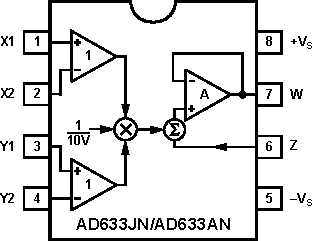
\includegraphics{Immagini/ad633_pinout.pdf}
		\caption{PinOut e schema a blocchi dell'AD633}
		\label{fig: AD633 schema a blocchi}
	\end{figure}


\chapter{Scelte progettuali}
	\label{ch:scelte}
	
	Nella realizzazione di questo progetto si deve prestare particolare attenzione allo spettro del segnale di uscita. Nello specifico, si deve valutare la distorsione armonica totale ($THD$) della sinusoide di uscita osservando quanto le armoniche indesiderate, anche generate da disturbi intrinsechi del sistema, influiscano sulle performance del dispositivo.
	Per ridurre l'effetto di armoniche a frequenza esterna alla banda udibile si è scelto di introdurre cascate di filtri passa alto e passa basso in modo da cercare un insieme di filtri passa-banda che producano un effetto accettabile per l'esperienza. Di seguito è riportato lo schema a blocchi del sistema:

	\begin{figure}[h]
		\centering
		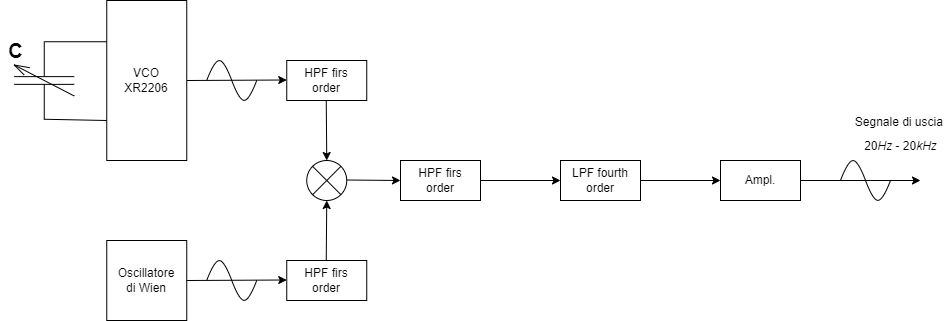
\includegraphics[scale=0.5]{Immagini/Schema a blocchi PSEA.png}
		\caption{Schema a blocchi del sistema realizzato}
		\label{fig: Schema a blocchi finale}
	\end{figure}
\space
	\noindent Nelle sezioni successive vengono analizzate singolarmente le scelte effettuate per ogni singolo blocco del sistema.
	 
\section{VCO}

	Il VCO, \textit{Voltage Controlled Oscillator}, è un generatore di segnali che modifica la frequenza di oscillazione del segnale generato in funzione della tensione applicata al suo ingresso.
	
	\noindent In relazione all'integrato utilizzato, il cui schema interno è riportato in figura \textit{Figura \ref{fig:sch_xr2206_}}, la frequenza di oscillazione $f_0$ viene controllata da una capacità esterna C, detta capacità di $timing$ collegata tra i \textit{pin5} e $pin6$ e dalla resistenza R posta in ingresso ai $pin7$ e $pin8$. Essa viene calcolata come:
	
	\begin{equation}
		\label{eq:freq_operation}
		f_0 = \frac{1}{RC} 
	\end{equation}

	\noindent Regolando il valore di \textit{R}, dato dalla somma di $R_1 + 1k\Omega$, e di \textit{C}, si imposta a piacere la frequenza di oscillazione.
	Nel progetto si è scelto di utilizzare una resistenza \textit{R} fissa in quanto si ha una capacità variabile per la regolazione della frequenza.

	\begin{figure}[h]
		\centering
		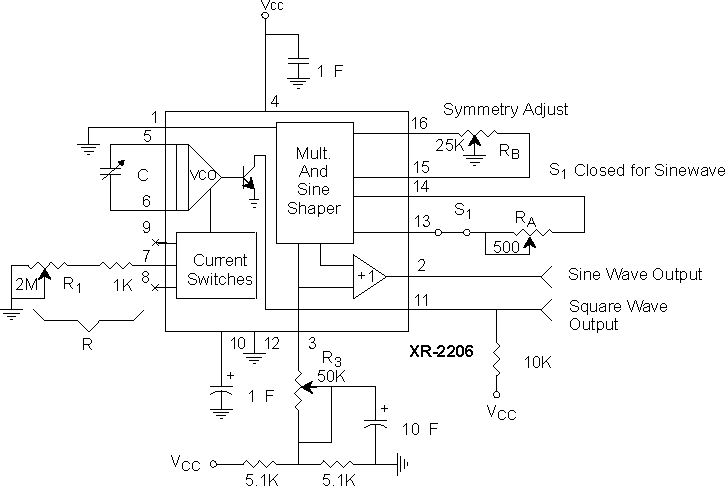
\includegraphics[scale=1]{Immagini/schema_xr2206.pdf}
		\caption{Schema a blocchi interno dell'oscillatore monolitico XR2206}
		\label{fig:sch_xr2206_}
	\end{figure}
	\newpage

	\noindent
	Dal datasheet, per garantire una buona stabilità in temperatura, viene consigliato di utilizzare valori di R compresi tra $4k\Omega < R < 200k\Omega$ e valori di C compresi tra $1\mu F < C < 100\mu F$.
	
	\noindent Dal momento che la capacità risulta variabile, in quanto dipendendente dalla posizione della mano dell'utente e dalla geometria dell'antenna realizzata, si è scelta una R di $100k\Omega$ per cercare di rispettare, almeno in parte, il range fornito dal datasheet per garantire una buona stabilità in temperatura. 
	
	% Inserire lo studio del THD generato dal VCO 
	
\section{Oscillatore sinusoidale di Wien}
	\label{sec:osc_wien}
	Per la realizzazione di un segnale sinusoidale a frequenza fissata si è scelto di utilizzare un oscillatore a ponte di Wien auto-avviante, il cui schema è riportato in \textit{Figura \ref{fig:sch_osc_wien}}
	
	\begin{figure}[h]
		\centering
		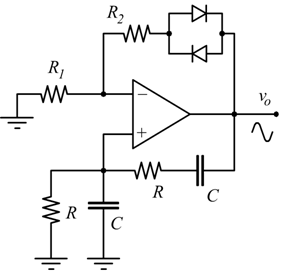
\includegraphics[scale=0.7]{Immagini/sch_osc_wien.png}
		\caption{Schema generale di un oscillatore a ponte di Wien auto-avviante.}
		\label{fig:sch_osc_wien}
	\end{figure}

	\noindent Analizzando la $f.d.t$ del circuito si osserva che il prodotto $A\cdot B$ deve essere 1, quindi un numero reale.
	Il blocco di forward A è rappresentato dal guadagno del circuito ovvero: 

	\begin{equation}
		\label{eq:LF356_Gain}
		A = 1 + \frac{R_2}{R_1}
	\end{equation}


	Mentre, in presenza di $R$ e $C$ di valore unico, il blocco di feedback B è rappresentato dall'equazione:
	\\
	\begin{equation}
		\label{eq:LF356_Feedback}
		B = \frac{1}{3 + j\omega C R - j\frac{1}{\omega C R}}
	\end{equation}
	\\
	Per l'innesco delle oscillazioni è necessario che il guadagno ad anello aperto sia inizialmente $A\cdot B>1$ ed $A>3$ per poi assestarsi a $A\cdot B=1$ ed $A=3$. La tecnica più semplice consiste nel disporre due diodi in antiparallelo lungo l'anello di retroazione dell'OpAmp.
	
	\noindent Quando \textit{$V_{O}$} è bassa i diodi presentano un'alta resistenza differenziale mentre all'aumentare di \textit{$V_{O}$} essa diminuisce. 
	\\ Per rispettare le condizioni di lavoro imposte, il guadagno A può essere posto, circa, all'85\% del suo valore nominale (A=2,5 — 2,55) così si fa in modo modo che $A>3$ all'avvio che poi si riduce ad A=3 a regime.

	\begin{figure}[H]
		\centering
		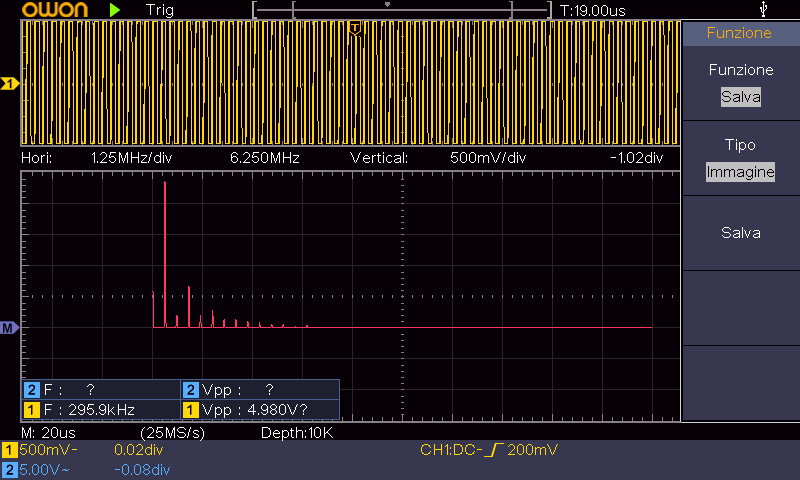
\includegraphics[scale=0.9]{Immagini/009_OscillatoreWienFFT.png}
		\caption{FFT della sinusoide a 295kHz in uscita dall'oscillatore acquisita tramite oscilloscopio}
		\label{fig:FFT295k}
	\end{figure}
	
	%Dalla \textit{Figura \ref{fig:FFT295k}} si può notare la presenza di sole due armoniche: quella voluta a 295kHz e una componente in continua. \\
	%La componente in continua è sicuramente dovuta alla strumentazione utilizzata poiché anche introducendo un elemento capacitivo per disaccoppiare, la componente è sempre rimasta presente.
	Per la valutazione della distorsione della sinusoide ottenuta si utilizza il calcolo del THD riportato nell'equazione:
	
	\begin{equation}
		\label{eq:thd}
		THD (\%) = 100 \cdot \frac{\sqrt{\sum_{2}^{\infty} V_{n}^2}}{V_1}
	\end{equation}

	Tutti i valori di tensione devono essere in RMS: 
	
	\begin{equation}
		\label{eq:Vrms}
		V_{RMS} = \frac{V}{\sqrt{2}}
	\end{equation}

	La presenza di un THD più o meno buono si manifesta con un andamento della sinusoide di uscita più o meno ideale. L'aggiunta di nuove armoniche poù essere cuasata dalla sensibile alle temperature dell'oscillatore di Wien, che porta anche ad una variazione delle ampiezze. Un'altra possibile fonte di diturbi e/o distorioni potrebbe essera la saturazione dell'amplificatore utilizzato per realizzare l'oscillatore, oltre che altre fonti esterne.


	% Se la distorsione non è armonica cosa succede? Ottendo piu righe spettrali che mi generano disturbi nel segnale
	
	% Cosa succede se la distorsione è sull'amplificatore, piuttosto che sull'oscillatore piuttosto che sull'XR? Bisogna che i componenti siano a bassa distorsione armonica.
	
	% Se il segnale in uscita all'oscillatore di wien fosse triangolare, cosa accade dopo il motiplicatore? Prossima lezione si vedrà cosa accade se il segnale è un onda quadra.
		
\newpage
\section{Moltiplicatore analogico}
	Alla moltiplicazione di due segnali nei tempi corrisponde la convoluzione degli stessi in frequenza. Questo porta ad ottenere due sinusoidi centrate a frequenza $\omega_1 + \omega_2$ e $\omega_1 - \omega_2$.
	
	\noindent In \textit{Figura \ref{fig:FFTmixer}} viene mostrato il risultato ottenuto moltiplicando la sinusoide ottenuta precedentemente \textit{Sezione \ref{sec:osc_wien}} con l'oscillatore di Wien, avente una $\omega_0$ di 45kHz, e una sinusoide generata dal generatore di funzione ad una frequenza di 20 kHz.

	\begin{figure}[H]
		\centering
		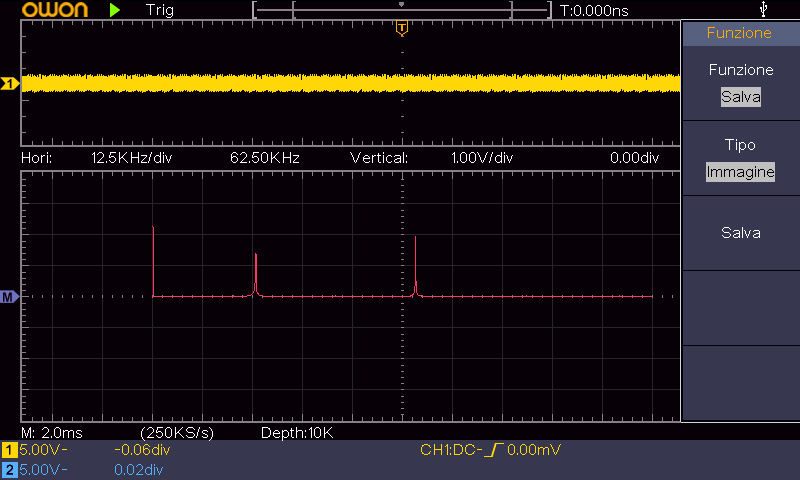
\includegraphics[scale=0.9]{Immagini/uscita_ad633_con_fcngen_20k_e_osc_45k.png}
		\caption{FFT del segnale in uscita dall'AD633, con test tra Oscillatore di Wien avente $\omega_0$ = 45kHz 12V picco e generatore di funzione con segnale 20 Khz e 2.5V picco.}
		\label{fig:FFTmixer}
	\end{figure}
	
	 \noindent Essendo i due segnali in gioco di 20kHz e 45kHz, dalla  \textit{Figura \ref{fig:FFTmixer}} si può notare come vengano generate due sinusoidi aventi armoniche fondamentali a $(45-20)kHz$ e $(45+20)kHz$. %escludendo la componente armonica a frequenza nulla che è generata dalla strumentazione come spiegato in precedenza.
	 \\
	 Inoltre, le ampiezze rilevate risultano in linea con i risultati teorici in quanto l'ampiezza di picco dei due segnali in gioco è di $12V$ e $2.5V$ rispettivamente, che vengono moltiplicate tra loro e divise di un fattore $10$ come specificato nel datasheet del componente. Si nota anche come le due ampiezze non siano uguali: questo è un errore dovuto alla non-linearità del componente. Tuttavia, per la nostra applicazione questo errore è irrilevante in quanto interessa maggiormente la componente armonica del segnale.
	

\section{Filtro LP del quarto ordine}
	Il prodotto di due sinusoidi del mixer porterà in uscita due sinusoidi a frequenze diverse ovvero una sarà $\omega_{wien} + \omega_{VCO}$ e l'altra a $\omega_{wien} - \omega_{VCO}$. Per rientrare nelle specifiche di progetto, è stato necessario introdurre un filtro passa-basso (LP) tale che permettesse di avere in uscita solo la componente armonica $\omega_{wien} - \omega_{VCO}$.
	\\ 
	Volendo un filtro molto selettivo e visto che il compondente $LF353P$ ha al suo interno due amplificatori, si è scelto di utilizzare un filtro attivo di ordine 4. Realizzandolo tramite un filtro di Chebychev con due celle Sallen-Key in casacata. 
	
	\begin{figure}[H]
		\centering
		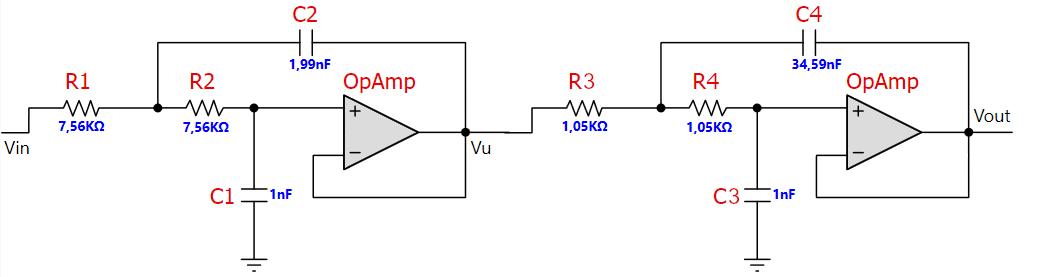
\includegraphics[scale=0.9]{Immagini/sch_lp4.png}
		\caption{Filtro attivo di ordine 4.}
		\label{fig:LP4}
	\end{figure}	
	
	\noindent Dove la sua risposta teorica in frequenza del modulo del filtro risulta essere quella riportato nel diagramma di Bode mostrato in \textit{Figura \ref{fig:BodeLp4}}.
	
	\begin{figure}[H]
		\centering
		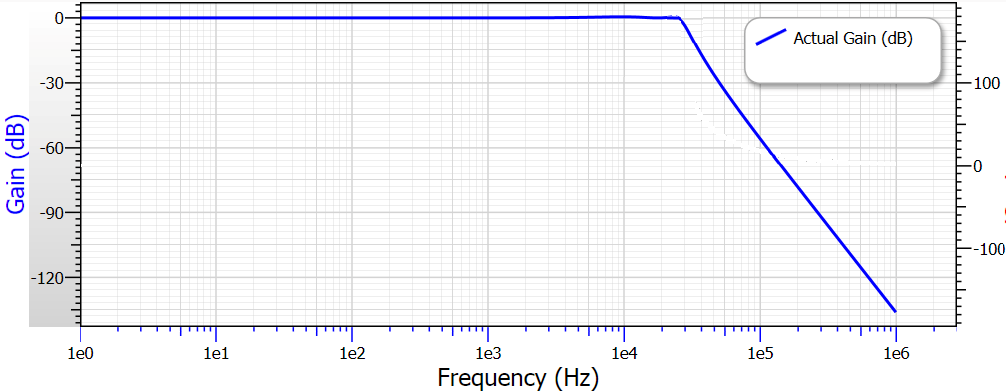
\includegraphics[scale=0.9]{Immagini/bode_teorico_lp4.png}
		\caption{Diagramma di Bode del modulo del filtro.}
		\label{fig:BodeLp4}
	\end{figure}

	La funzione di trasferimento del filtro del quarto ordine può essere visto come il prodotto in cascata delle funzioni di trasferimeto delle due celle Sellen-Key del secondo ordine.
	La funzione della prima cella risulta:

	\begin{equation}
		H_1(s) = \frac{V_{in}}{V_u}  =  \frac{1}{1 + sC_1(R_1 + R_2)+ s^2C_1C_2R_1R_2 } 
	\end{equation}

	Mentre la funzione di trasferimento della seconda cella risulta essere:

	\begin{equation}
		H_2(s) = \frac{V_u}{V_{out}}  = \frac{1}{1 + sC_3(R_3 + R_4)+ s^2C_3C_4R_3R_4 } 
	\end{equation}

	La funzione di trasferimento totale del filtro sarà data dal prodotto delle due funzioni di trasferimento
	\begin{equation}
		H(s) = H_1(s)H_2(s) =  \frac{V_{in}}{V_u}\frac{V_u}{V_{out}} = \frac{V_{in}}{V_{out}}
	\end{equation}

	



\chapter{Risultati sperimentali}

\section{XR2206}
	Per la realizzazione dell'armonica a frequenza variabile ci siamo appoggiati al datasheet del componente scegliendo come valori di partenza quelli mostrati in esempio. 
	
	La capacità variabile è stata realizzata con un supporto rigido e della carta di alluminio posta a bandiera. Il tutto è stato collegato come mostrato in figura.
	
	% TODO:inserire foto circuito XR2206 con antenna.
	
	Le prestazioni ottenute con questo tipo di antenna sono le seguenti:
	
	% TODO: Foto distanza misurata della mano (senza mano, dove comicia a variare, variazione massima)

	\begin{figure}[H]
		\centering
		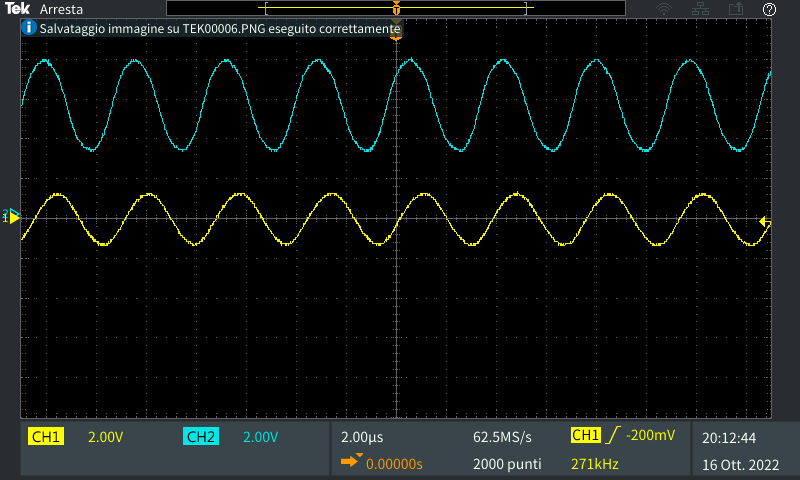
\includegraphics[scale=0.5]{Immagini/sin_xr+lp.PNG}
		\caption{Confronto tra i segnali in uscita dall'oscillatore monolitico XR2206 prima e dopo il fitro LP in cascata.}
		\label{fig:SINxr+LP}
	\end{figure}


	\begin{figure}[H]
		\centering
		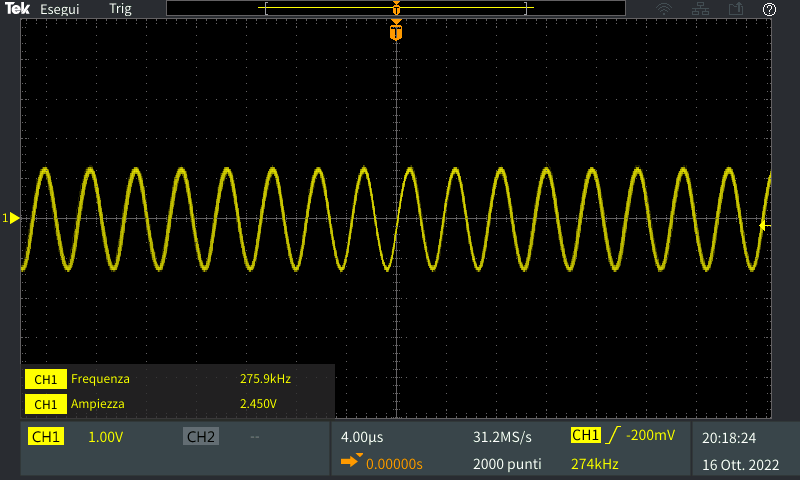
\includegraphics[scale=0.5]{Immagini/sin_xr.PNG}
		\caption{Segnale in uscita dal blocco XR2206 + LP.}
		\label{fig:SINx}
	\end{figure}

	\begin{figure}[H]
		\centering
		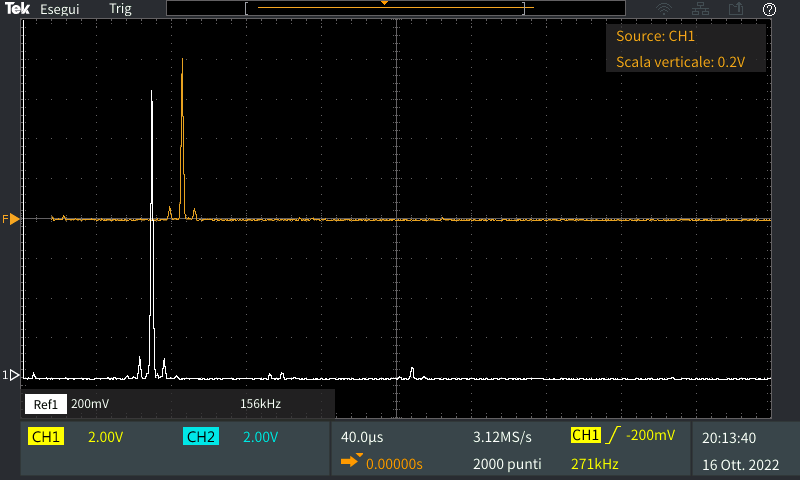
\includegraphics[scale=0.5]{Immagini/fft_xr+lp.PNG}
		\caption{Confronto tra le FFT del segnale in uscita dall'oscillatore monolitico XR2206 prima e dopo il filtro LP in cascata.}
		\label{fig:FFTxr+LP}
	\end{figure}




	\begin{figure}[H]
		\centering
		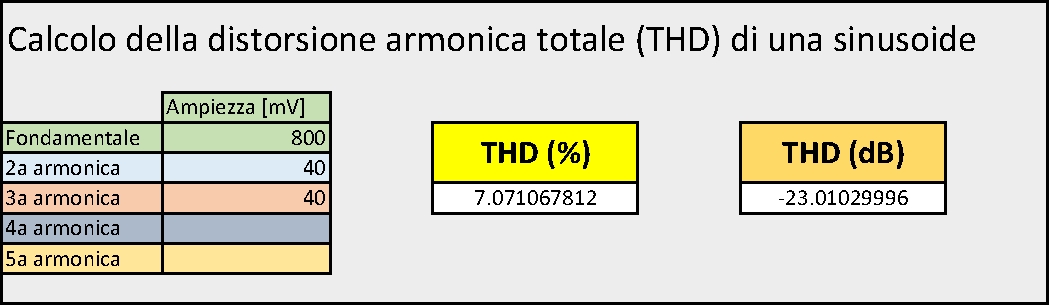
\includegraphics[scale =1]{Immagini/thd_xr+bp.pdf}
		\caption{THD dell'XR2206 dopo il passa banda}
		\label{fig:THDXR+BP}
	\end{figure}

\section{Oscillatore di Wien}

Il circuito finale utilizzato per realizare l'oscillatore di Wien è quello riportato in figura \ref{sch:osc_wien}.

\begin{figure}[H]
	\centering
	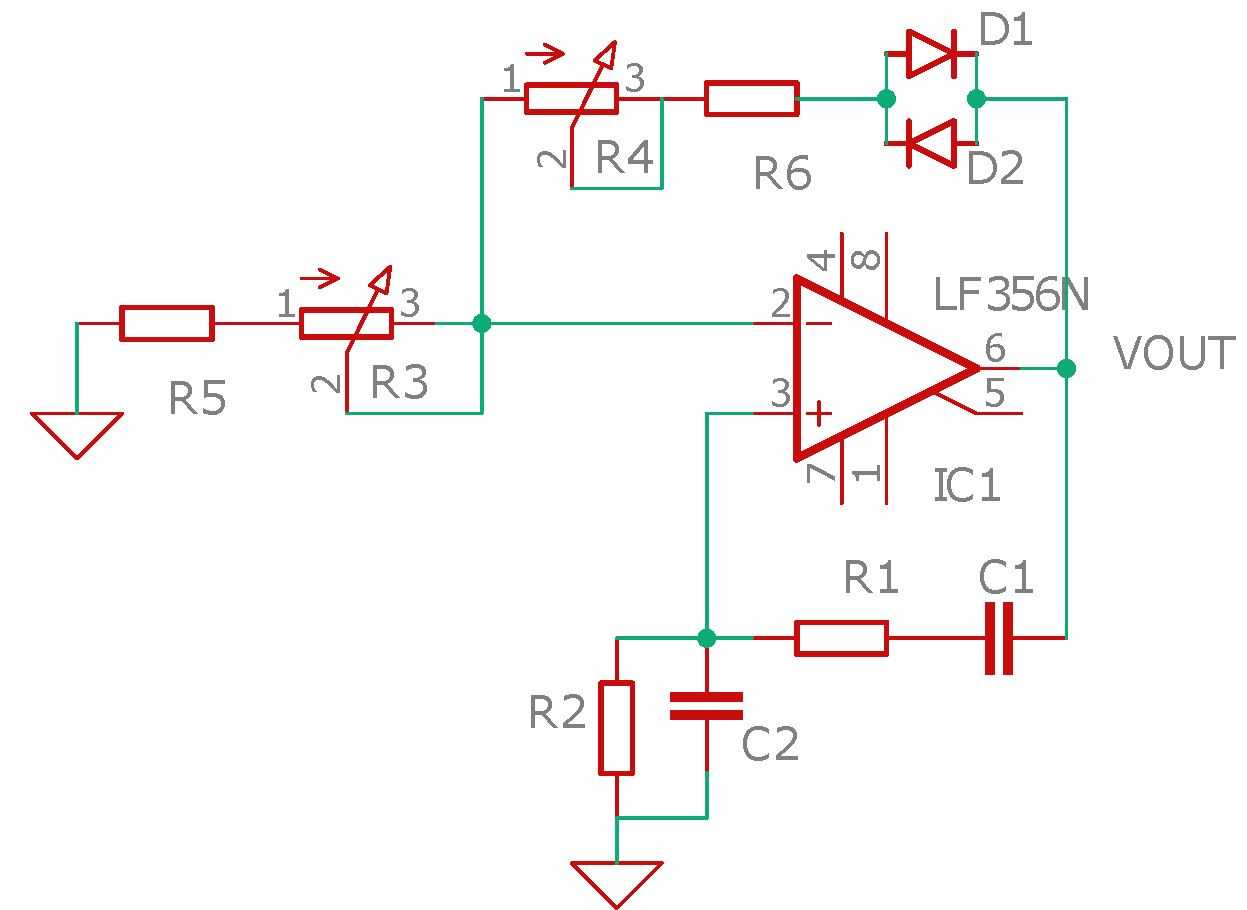
\includegraphics[scale=0.5]{Immagini/sch_osc_wien_cad.pdf}
	\caption{Schematico dell'oscillatore di Wien utilizzato}
	\label{sch:osc_wien}
\end{figure}

Si può notare che sono stati aggiunti due potenziometri, $R3$ e $R4$ rispettivamente, del valore  $1k\Omega$,  in serie alle resistenze $R5$ e $R6$ del valore di  $1k\Omega$. Tale scelta è stata fatta per accordare l'oscillazione del segnale e ridurre quindi la distorsione armonica. Tuttavia si è notato che la presenza di questi ultimi può portare alla perdita dell'oscillazione stessa, in quanto se i due potenziometri hanno valori simili l'oscillazione scompare. Grazie ai potenziometri, si ha la possibilità di sbilanciare il ponte rendendo possibile l'avviarsi dell'oscillatore ottenendo un'oscillazione stabile e con una possibilità di regolazione.

	\begin{figure}[H]
		\centering
		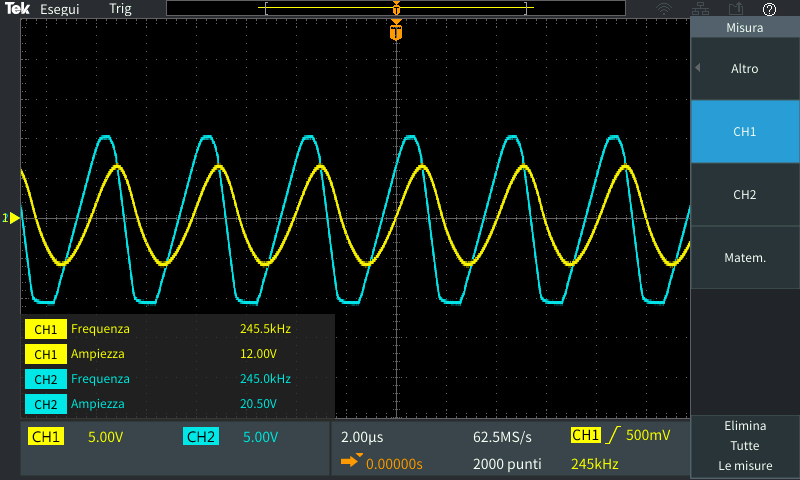
\includegraphics[scale=0.5]{Immagini/osc_wien+bp210k.PNG}
		\caption{Confronto tra i segnali in uscita dall'oscillatore di Wien prima e dopo il fitro BP in cascata.}
		\label{fig:SINwien+BP}
	\end{figure}

	La figura \ref{fig:SINwien+BP} mostra l'uscita dell'oscillatore di Wien. In azzuro si può notare che la sinusioide satura sulla parte negativa e la pendenza di salita a discesa sono differenti, questo è dovuto allo sbilanciamento dei due potenziometri. L'insieme di questi due fattori porta all'introduzione di altre armoniche oltre alla fondamentale, come mostrato in bianco nella figura \ref{fig:FFTwien+BP}.
	Per risolvere il problema è stato aggiunto un filtro passivo all'uscita dell'oscillare. Il filtro è di tipo passa banda formato da un condensatore per tagliare la continua, seguito da un passa basso RC ($R = 7.5k\Omega$; $C = 100pF; f_c = 212kHz$).
	L'aggiunta del filtro porta un sostanziale miglioramento della sinusoide d'uscita. Il miglioramento è visibile sia in figura \ref{fig:SINwien+BP}, sinusoide gialla, dove si vede l'assenza di saturazione e fronti di salita e discesa pressoché identici, che in figura \ref{fig:FFTwien+BP} dove di nota la notevole riduzione delle armoniche nello spettro del segnale.

	Tuttavia, l'aggiunta del filtro porta ad un'attenuazione anche dell'armonica fondamentale e ad uno sfasamento di 90° in ritardo rispetto alla sinusoide originale. L'attenuazione è dovuta alla scelta della frequenza di taglio del filtro ($212kHz$), quindi il filtro inizia a tagliare circa $20/30kHz$ prima della fondamentale dell'oscillatore di Wien che risulta essere a $245kHz$. Lo sfasamento invece è dovuto al filtro del primo ordine passivo.

	\begin{figure}[H]
		\centering
		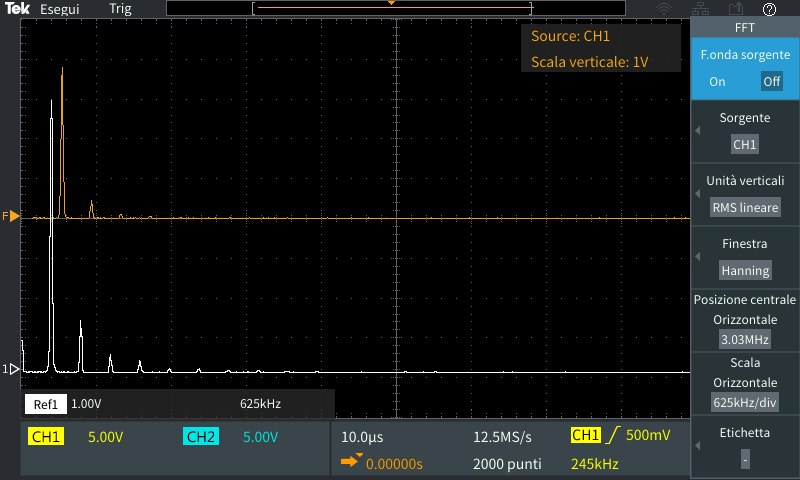
\includegraphics[scale=0.5]{Immagini/fft_osc+bp210k.PNG}
		\caption{Confronto tra le FFT del segnale in uscita dall'oscillatore di Wien prima e dopo il filtro BP in cascata.}
		\label{fig:FFTwien+BP}
	\end{figure}

	Un altro riscontro lo si ha con il calcolo del $THD$ del segnale in usscita dall'oscillatore. Il risultato calcolato con l'equazione \ref{eq:thd}, si può vedere della figura \ref{fig:ThdWien} dove si mostra il valore del $THD$ del segnale in uscita dall'oscillatore. In figura \ref{fig:ThdWien+lp} è riportato il valore del $THD$ dopo il filtro passa banda passivo. Si nota un effettivo miglioramento del $THD$ della sinusoide di riferiento.

	\begin{figure}[H]
		\centering
		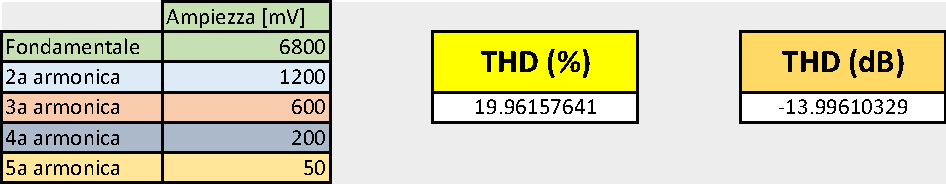
\includegraphics[scale=0.5]{Immagini/thd_osc.pdf}
		\caption{Valori delle armoniche ricavate dalla FFT del segnale in unscita dall'oscillatore di Wien.}
		\label{fig:ThdWien}
	\end{figure}
	 
	\begin{figure}[H]
		\centering
		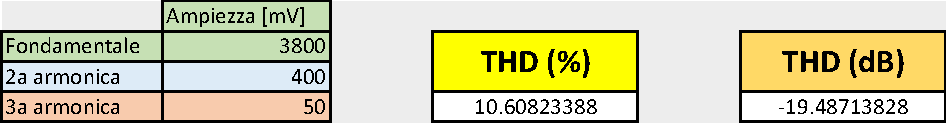
\includegraphics[scale=0.5]{Immagini/thd_osc+bp.pdf}
		\caption{Valori delle armoniche ricavate dalla FFT del segnale in unscita dall'oscillatore di Wien.}
		\label{fig:ThdWien+lp}
	\end{figure}


\section{Mixer}
\label{sec:Mixer}


L'AD633 rappresenta il blocco del mixer nel nostro sistema. Il suo compito è fare il prodotto tra due sinusoidi in ingresso. Le due sinusoidi sono quella di riferimento dell'oscillatore di Wien e quella in uscita dal VCO. Quest'ultima sarà variabile e dipenderà dalla distanza della mano rispetto all'altro estremo della capacità variabile (banderuola in alluminio). Il circuito dell'oscillatore è mostrato in figura xxxx


Una delle problematiche riscontrate durate l'utilizzo del mixer è stata la comparsa di un offset in continua dovuto all'impossibilità degli ingressi di scaricare le correnti di bias, correnti in continua, verso massa. Questo ha portato alla comparsa di offset negativo e allo smorzamento delle altre armoniche presenti in uscita, come mostra la figura xyz.



Il problema è stato risolto ponendo una resistenza di valore $680k\Omega$ agli ingressi del mixer e portandoli verso massa. La scelta di tale valore è stata condizionata dal fatto che si deve garantire un compromesso tra l'ingresso ad alta impedenza dell'AD633 e il partitore che si forma con la resistenza del filtro che produrrebbe un'attenuazione del segnale in ingresso. Il resistore scelto evita un'attenuazione del segnale e salvaguarda l'alta impedenza del componente. Il risultato è mostrato in figura blabla. Dove è possibile vedere le due armoniche fondamentali che vengono a formarsi dal prodotto di due sinusoidi, esattamente come ci si aspetta dalla teoria. Cosa che non accade in figura xyz, ovvero prima che venissero messe le resistenze.
	
	%Verificare il limiti operativi del componente.
	
	%Verifichiamo il THD delle sinusoidi in uscita dall'Oscillatore e AD633 	Osserviamo che in entrambi i casi non otteniamo distorsioni. Notiamo una continua di circa 2V che non riconosciamo. 	Aggiungendo un condensatore di filtraggio in uscita al moltiplicatore non otteniamo risultati. Ipotizziamo sia dovuto a qualcosa di intrinseco all'oscilloscopio.  	Anche perché nella visualizzazione della sinusoide non rileviamo alcun offset. Inoltre ad un certo punto delle misurazioni è sparito. 	Abbiamo osservato che l'ampiezza delle righe della fft è coerente con i segnali in ingresso al sistema. $V_{osc}$=15V $V_{fcngen}$=2.5V quindi considerando il fattore intrinseco di scala dell'AD633 otteniamo delle righe di fft di ampiezza coerente perché sommando le varie componenti si ottiene quei 3.5V circa di ampiezza del segnale.

	\begin{figure}[H]
		\centering
		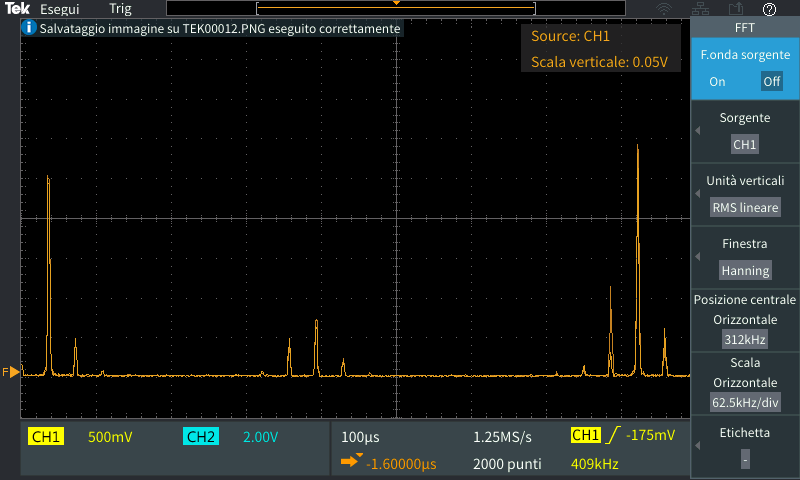
\includegraphics[scale = 0.5]{Immagini/ad633_fft_mixed.PNG}
		\caption{FFT in sucita dal mixer AD633 senza filtraggio}
		\label{fig:FFTAD633}
	\end{figure}

	%\begin{figure}[h]
		%\centering
		%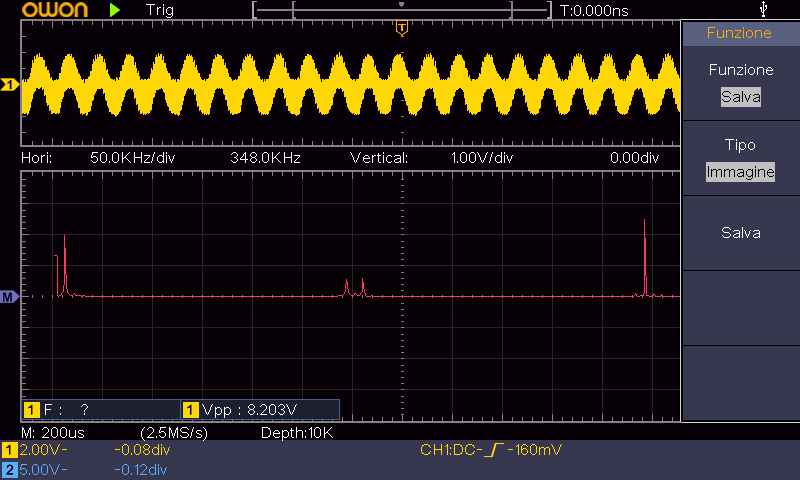
\includegraphics[scale=0.9]{Immagini/AD633_300k.png}
		%\caption{FFT in uscita dall'AD633 con fondamentale a %300k}
	%	\label{fig:FFTAD633}
	%\end{figure}

	\label{ch:Risultati}
	
	% TODO: Qui tutta la pappa con le immagini oscilloscopio e breadboard, qualche calcolo anche excel e tanta ma tanta descrizione che non serve a nulla

\newpage
\section{Filtro passa basso di ordine 4}
	In uscita dal mixer è stato necessario inserire un filtro passa basso per eliminare le frequenze superiori ai $20kHz$, come richiesto da specifica di progetto. Esso è necessario per eliminare le componenti date dalla somma delle frequenze in uscita al mixer risultanti dell'equazione. Infatti, dati due segnali del tipo $ V_1 = A_1 \cdot sin(\omega_1t) $
	e $ V_2 = A_2 \cdot sin(\omega_2t) $, il segnale risultante dalla moltiplicazione analogica tra i due sarà dato dall'equazione \ref{eq:analog_multiply}:
	\begin{equation}
		V_m = V_1 \cdot V_2 = \frac{A_1A_2}{2}[sin((\omega_1 + \omega_2)t) + sin((\omega_1 - \omega_2)t)]
		\label{eq:analog_multiply}
	\end{equation}
	La figura \ref{fig:bode_LF353P} mostra il comportamento in frequenza dell'LF353P, ovvero il componente utilizzato per la realizzazione del filtro passa basso di ordine quattro.

	\begin{figure}[h]
	     	\centering
	     	\subfloat[][\emph{Didascalia figura }]
	     	{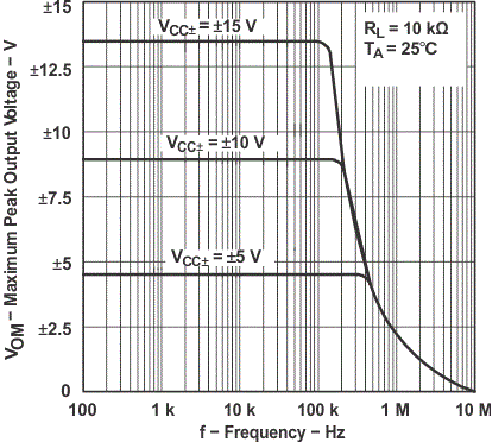
\includegraphics[width=.45\textwidth]{Immagini/lf353p_performance.pdf}} \qquad
	     	\subfloat[][\emph{Didascalia figura}]	     	{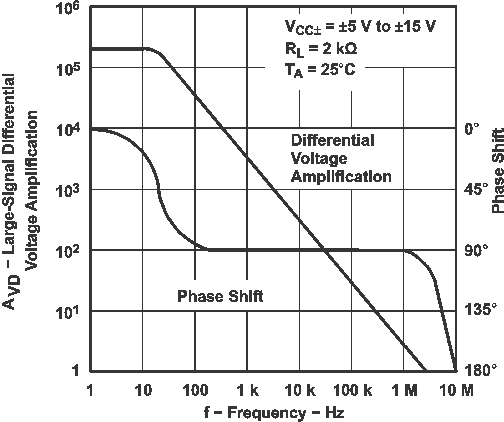
\includegraphics[width=.49\textwidth]{Immagini/bode_lf353p.pdf}} \\
	     	\caption{Diagrammi di bode del componente LF353P in anello aperto}
	     	\label{fig:bode_LF353P}
	     \end{figure}

	La scelta di un filtro del quarto ordine è stata fatta sia per garantire un'atteuazione sufficiente delle armoniche successive ai $20kHz$ sia perché l'LF353P contiene al suo interno due operazionali. Quindi per evitare di lasciare flottanti dei pin che sarebbero potuti diventare una fonte aggiuntiva di rumore, si è deciso di utilizzare il componente al meglio delle possibilità.
	L'andamento del filtro ottenuto è mostrato in figura \ref{fig:BODELp4Real}, la quale mostra che le scelte progettuali sono state corette, in quanto i dati sperimentali rispecchiano l'andamento teorico del filtro.
	Come si può osservare in figura \ref{fig:BODELp4Real} i due andamenti sono molto simili.
	
	\begin{figure}[h]
			\centering
			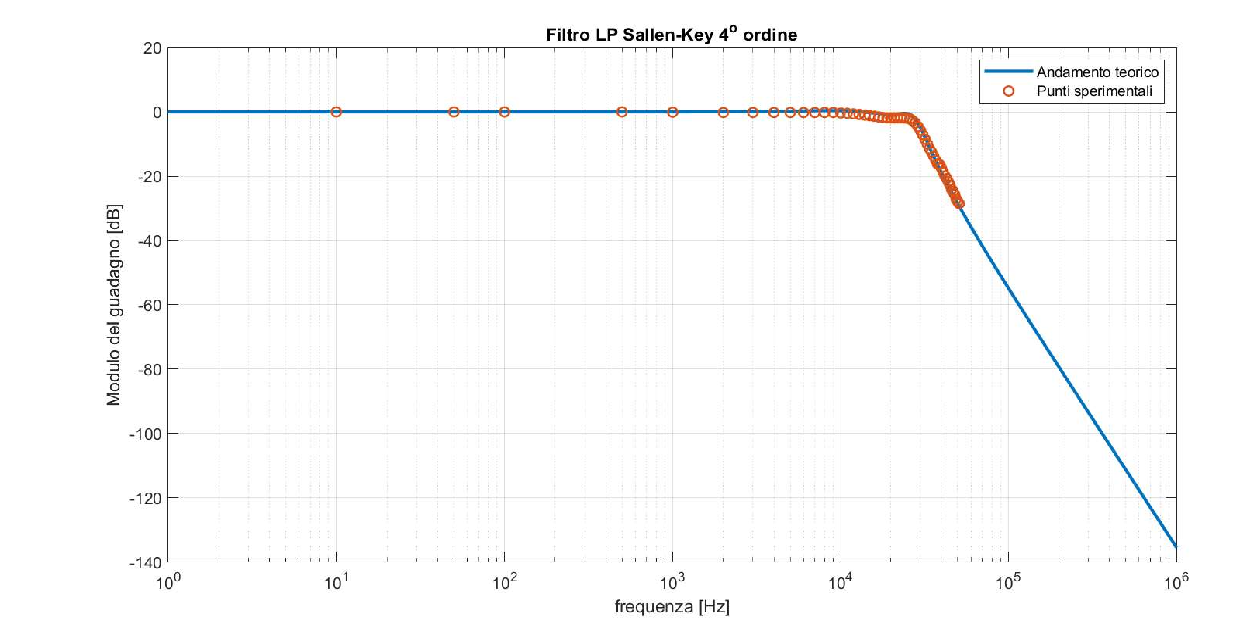
\includegraphics[scale=0.7]{Immagini/bode_lp4.pdf}
			\caption{Diagramma di Bode del filtro Sallen-Key del $4^o$ ordine}
			\label{fig:BODELp4Real}
		\end{figure}
	
	
	% TODO: Inserire un diagramma per punti mettendo in ingresso al filtro un segnale con il generatore di funzioni variando la F di X kHz e visualizzando l'uscita sull'oscilloscopio
	%\subsection{Analisi della banda in anello chiuso}
	     

		
     	% TODO: Testare il filtro passa alto che porta essere posizionato o in fondo prima o dopo del 741, oppure tra il mixer e il filtro del 4o ordine.
     	
     	%% Conti sul rumore non ce ne servono   

\newpage
\section{Filtro passa altro del primo ordine}
		Qua dentro ci mettiamo: \\
		datasheet \\
		Circuito \\
		Risposta in frequenza bode \\
		Giustificare che taglia a 10k perchè la banda passante dell'ampli fa schifo \\

		In mancanza di componenti abbiamo dovuto adattarci
		( in teoria ampli sposta bode)

		\begin{figure}[H]
			\centering
			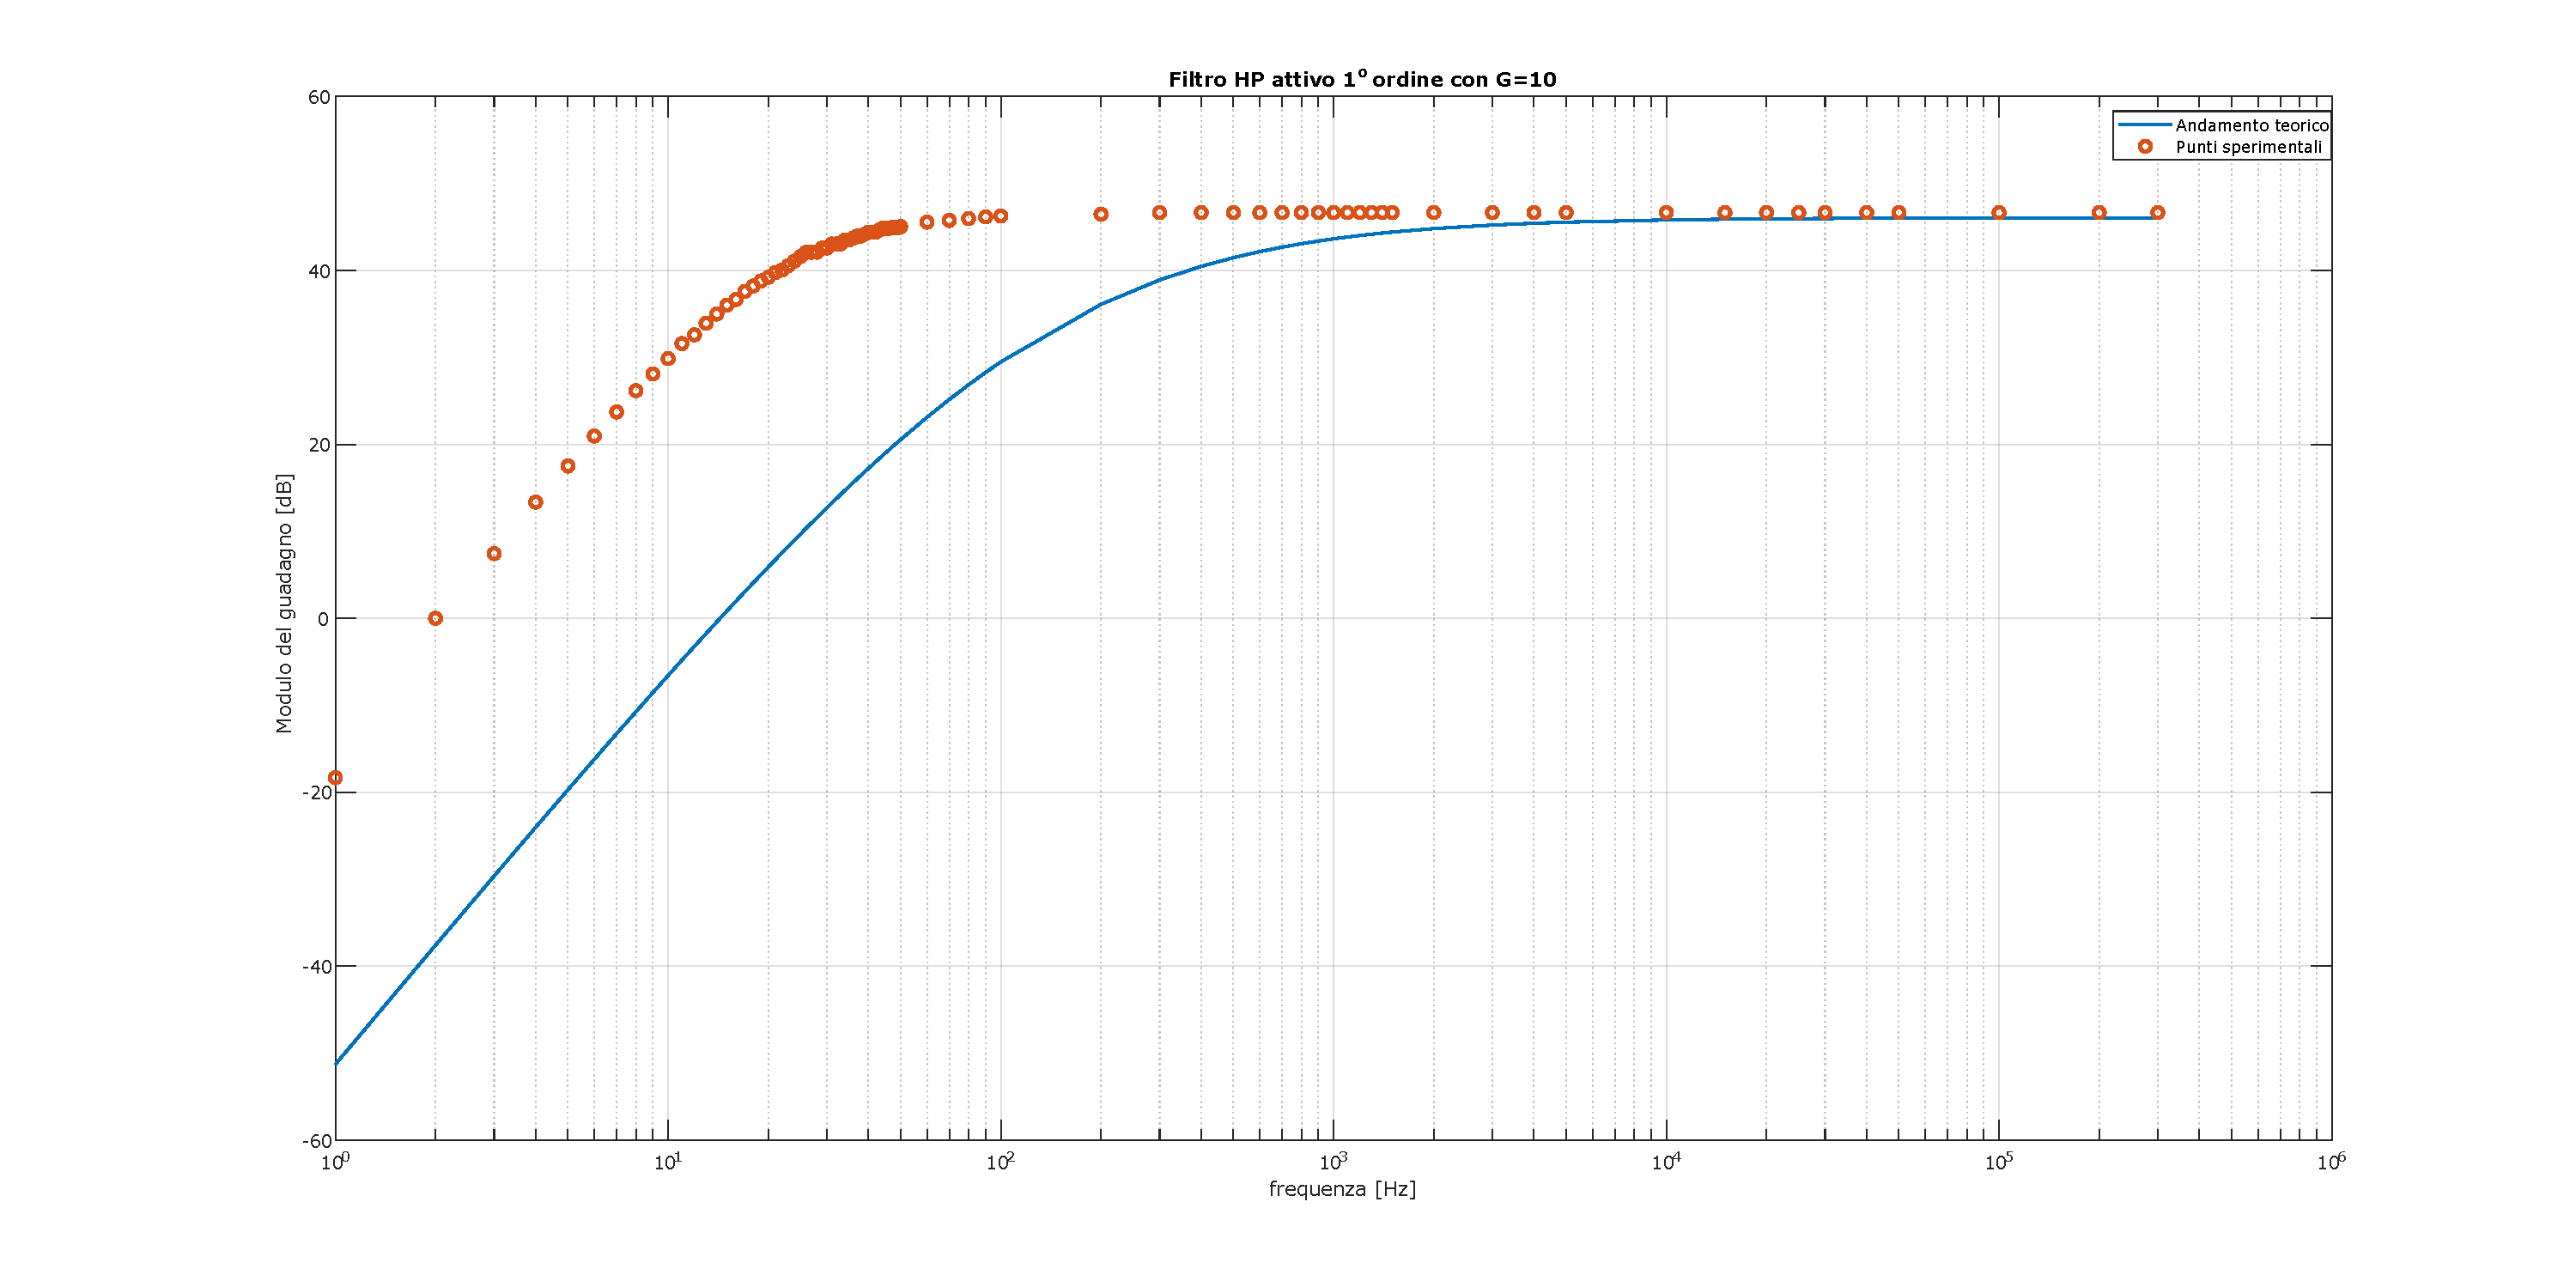
\includegraphics[scale=0.34]{Immagini/bode_hp1_ua741.pdf}
			\caption{Diagramma di Bode del filtro passa alto del $1^o$ ordine}
			\label{fig:BODEHp1Real}
		\end{figure}

\section{Theremin}
\label{ch:Teremin}
	%Schematico con cad
	In FIGURA PINCO PALLO è riportato lo schema circuitale completo del Theremin. Si possono vedere i vari blocchi spiegati nei capitoli precendeti come vengo fatti comunicare tra loro.

	La FIGURA PINCOPALLO VIVO mostra il circuito fisico realizzato per l'esperimento su cui si sono effettuate tutte le misurazioni.


	La scelta delle frequenze operative nell'ordine delle centinaio di $KHz$ è stata obbligata per potre avere una risoluzione accettabile in frequenza avvicinando la mano alla capacità variabile collegata al $VCO$.
	Come si è visto nelle sezioni precedenti e come è riportato nella figura \ref{fig:FFTwien+BP} e in figura \ref{fig:FFTxr+LP}.

	Altro passo obbligato è stato l'inserimento del filtro passa basso del quarto ordine in cascata al mixer. Questo ha portato ad un notevole miglioramento del THD del segnale in uscita, come mostra la FFT riportata in figura \ref{fig:FFTAD33+LP4}. Nella quale si può notare la presenza di una singola armonica. Ovvero lìoscilloscopio utilizzato non ha permesso di rilevare altre armoniche con la scala impostata. Quindi non c'è stato bisogno di calcoare il $THD$ del segnale.
	
	\begin{figure}[H]
		\centering
		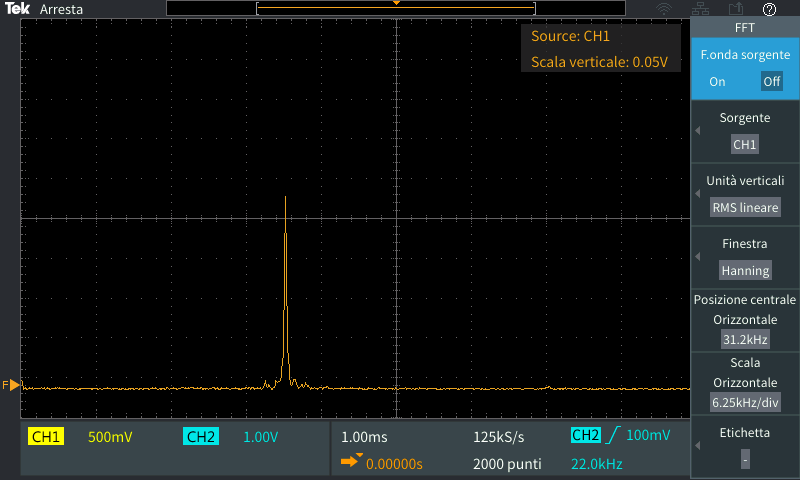
\includegraphics[scale = 0.5]{Immagini/fft_ad633+lp4.PNG}
		\caption{FFT in uscita dall'AD633 dopo il Filtro passa basso del quarto ordine}
		\label{fig:FFTAD33+LP4}
	\end{figure}

	L'aggiunta del filtro attivo passa alto è stato introdotto per taglaire la continua e le armoniche inferiori ai $20Hz$.
	In figura \ref{fig:FFTfinale}.


	\begin{figure}[H]
		\centering
		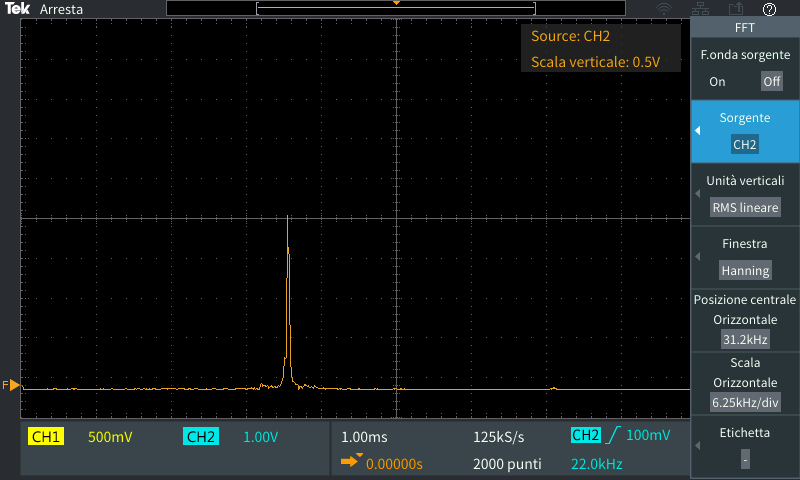
\includegraphics[scale = 0.5]{Immagini/ftt_ad633+lp4+hp1_final.PNG}
		\caption{FFT della sinusoide in uscita dal sistema}
		\label{fig:FFTfinale}
	\end{figure}


	 La differeza tra le due è poco apprezzabile della $FFT$, ma si può notare in figura \ref{fig:AD33+LPconsenzaHP} che la sinusioide gialla, quella in uscita al filtro passa basso del quarto ordine, abbia delle componenti in ala frequezna evienziate dagli spike che si vedono sovrapposti alla sinusoide principale. Questi vengono eliminati dallo stadio successivo, ovvero il passa alto attivo. Questo perchè il passa alto è stato realizzato utilizzando come amplificatore operazione l'UA741, che ha un rapporto guadagno banda che cala in modo porporzionale al guadagno impostato dall'amplificatore, come spiegato \ref{sec:OpAmp}. Quindi da filtro passa alto teorico si ottiene un passa banda che va ad eliminare le coponenti in alta frequenza.
	 
	 \begin{figure}[H]
		\centering
		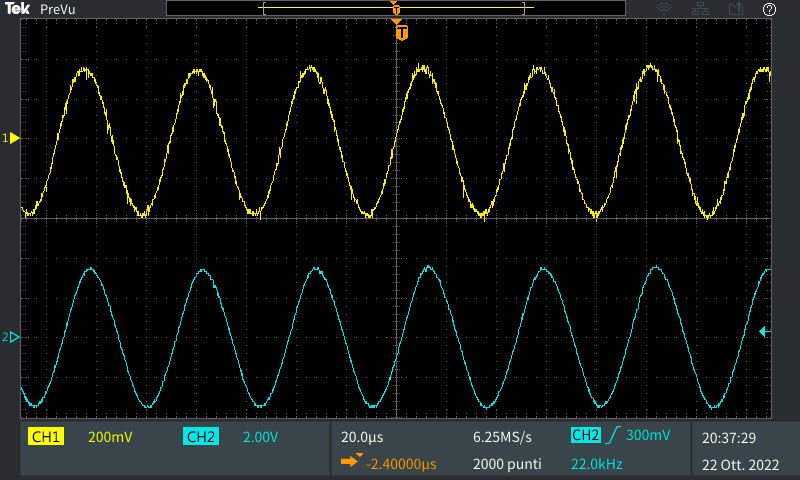
\includegraphics[scale = 0.5]{Immagini/sin_ad633+lp4_ad633+lp4+hp1.PNG}
		\caption{Sinusoidi in uscita dall'AD633 senza e con il filtro passa alto}
		\label{fig:AD33+LPconsenzaHP}
	\end{figure}


	La variazione di frequenza si manifesta con l'avvicinamento o l'allontanamennto della mano dell'utente dalla bandiera, che rappresenta l'altra faccia della capacità variabile. La variazione di capacità determinata dalla posizione della mano determina quindi la variazio di frequeza. Come primo tentativo avevamo deciso di utilizzare una frequenza di rifetminto di di $45KHz$ per poi var variare il segnale generato dal $VCO$ a frequenza che andassero da circa $45KHz$ a circa $85KHz$.
	Tuttavia, è stato riscontrato subito il problema della sensibilità.Ovvero si è visto che le uniche variazioni di frequenza apprezzabili si avevano quando la mano era a contatto con l'antenna o se questa era assente. Senza però portare le variazioni volute, si andava a coprire una piccolissima parte del range richiesto dal progetto.
	Quindi, si è deciso di alzare le frequeze operative, portando il riferimeno in uscita dall'oscillatore di Wien ad un valore di $245KHz$ come mostrato in figura \ref{fig:SINwien+BP}. Questo ha porta a dover aumentare anche il range di frequenze del $VCO$ portando così gli estremi da un'oscillazione di $275KHz$ senza mano a circa un $250KHz$ con la mano ad una distanza minima ove la mano risulta a contatto con l'atenna.
	Questa volta si è riscontranto un netto miglioramento della sensibilità nella variazione della frequeza rispetto alla distanza della mano.
	%Considerazioni sul circuito: scelta della frequenza di oscillazione
	%che è stata cambiata perchè non riuscivamo a farla variare con la mano ecc...
	
%\section{Problematiche}

% Cosa succede se la distorsione è sull'amplificatore, piuttosto che sull'oscillatore piuttosto che sull'XR? Bisogna che i componenti siano a bassa distorsione armonica.
	
	% Se il segnale in uscita all'oscillatore di wien fosse triangolare, cosa accade dopo il motiplicatore? Prossima lezione si vedrà cosa accade se il segnale è un onda quadra.


	% L'xr2206 inserisce un offset grazie al quale riesce a far oscillare l'uscita, il ptenziomentro R3 serve a gestire tale oscillazione mandando in saturazione o meno, mentre R5 aggiusta le componenti armoniche.

	%\label{FIGURE}
	

	
	

	

\chapter{Conclusioni}
 	\label{ch:Conclusioni}
	Bene questo progetto si conclude qui, \textit{grazie a tutti!}
	




	


\end{document}
